\documentclass[a4paper,12pt]{article}
\usepackage[a4paper, total={180mm, 272mm}]{geometry}

\usepackage{fontspec}
\setmainfont[Path=fonts/, Extension=.ttf]{ipaexm}

\setlength\parindent{3.5em}
\setlength\parskip{0em}
\renewcommand{\baselinestretch}{1.247}

\usepackage{epic}
\usepackage{eepic}
\usepackage{xcolor}

\usepackage{graphicx}
\graphicspath{{images/}}

\begin{document}

\thispagestyle{empty}

\Large
\noindent \\
Motion Wind Ino\medskip
\par
\normalsize
絵に流線の効果を加えます\\
\par
作画アニメーションで、早い移動を表す美術描画方法を参考にしています。\par
ピクセルの RGB 値から明るいピーク部分をきっかけにして、\par
色で流れるような効果を加えます。\\
\\
-{-}- \ 入力 \ -{-}-\\
Source\par
処理をする画像を接続します。\\
Reference\par
Pixel 毎に効果の強弱をつけるための参照画像を接続します。\\
\\
-{-}- \ 設定 \ -{-}-\\
Direction\par
流線の方向を指定します。\par
方向は上(Up)下(Down)左(Left)右(Right)方向のみです。\par
初期値は右(Right)となります。\par
ここでの方向は、カメラから見た方向に固定されます。画像の傾\par
きが変わるような、画像の回転やカメラの Z 回転等々\par
(Geometry 変換)によって方向を傾けることはできないので、\par
ご注意ください。\\
\\
Dark\par
OFF で明るい部分に対する流線となります。\par
ON のときは暗い部分に対する流線になります。\par
初期値は OFF です。\\
\\
Alpha Rendering\par
Alpha チャンネルがあるときのみ有効なスイッチです。\par
OFF のときは、RGB 値の変化を Alpha 値でマスクします\par
ON で Alpha にも処理をします。\par
初期値は ON です。\\
\\
Length Min\\
Length Max\par
流線の長さを指定します。\par
単位はミリメートルです。\par
ゼロ以上の値で指定します。最大は1000です。\par
小数点以下の指定により、微妙な長短の変化がつきます。\par
違う値を与えると、その値の間で長さがランダムに変化します。

\newpage

\thispagestyle{empty}

\ \vspace{-0.2em}
\par
同じ値にすると、ランダムさはなくなり全体が同じ長さとなります。\par
初期値は Min(最小値)が0、Max(最大値)が18となります。\par
-{-}> \textquotedbl Motion Wind 図1 \ \ Length Wind\textquotedbl 参照\par
-{-}> \textquotedbl Motion Wind 図4 \ \ Force is 1 and Density is 1\textquotedbl 参照\par
-{-}> \textquotedbl Motion Wind 図7 \ \ Length Wind and Force is 10\textquotedbl 参照\\
\\
Length Bias\par
長さのランダムパターンの片寄りを変えます。\par
0.1から1.0の間の値だと、短いのが増え、\par
1.0を指定すると均等なランダムさとなり、\par
1.0から10.0の間の値では、長いのが増えます。\par
となります。\par
初期値は1です。\par
-{-}> \textquotedbl Motion Wind 図1 \ \ Length Wind\textquotedbl 参照\\
\\
Length Seed\par
長さのランダムパターンを変えます。\par
ゼロ以上の整数値で指定します。\par
同じ画像に同じ値を与えると、同じパターンを再現します。\par
違うパターンにしたいときは値をかえます。\par
たとえば、Fix のムービーで、流線のパターン変化が欲しいとき\par
は、フレームごとに、seed 値を変えます。\par
初期値は1としています。\\
\\
Force Min\\
Force Max\par
流れ始めの勢いを指定します。\par
0.1から1.0の間だと、すぐ減衰して弱い勢い、\par
1.0を指定すると勢いがリニアに減衰し、\par
1.0から10.0の間では、なかなか減衰ぜず強い勢い、\par
となります。\par
違う値を与えると、その値の間で勢いがランダムに変化します。\par
同じ値にすると、ランダムさはなくなり全体が同じ勢いとなります。\par
初期値はどちらも1です。\par
-{-}> \textquotedbl Motion Wind 図2 \ \ Force Wind\textquotedbl 参照\par
-{-}> \textquotedbl Motion Wind 図5 \ \ Force is 0.1\textquotedbl 参照\par
-{-}> \textquotedbl Motion Wind 図7 \ \ Length Wind and Force is 10\textquotedbl 参照\\
\\
Force Bias\par
勢いのランダムパターンの片寄りを変えます。\par
0.1から1.0の間の値だと、弱いのが増え、\par
1.0を指定すると均等なランダムさとなり、

\newpage

\thispagestyle{empty}

\ \vspace{-0.2em}
\par
1.0から10.0の間の値では、強いのが増えます。\par
となります。\par
初期値は1です。\par
-{-}> \textquotedbl Motion Wind 図2 Force Wind\textquotedbl 参照\\
\\
Force Seed\par
勢いのランダムパターンを変えます。\par
以下\textquotedbl Length Seed\textquotedbl と同様です。\\
\\
Density Min\\
Density Max\par
流線の濃度を指定します。\par
ゼロだと流線効果がなくなり、\par
ゼロから1.0の間の値だと、うすくなり、\par
1.0のときは基準濃度で、\par
1.0より大きな値では、濃くなります。最大は100です。\par
違う値を与えると、その値の間で濃度がランダムに変化します。\par
同じ値にすると、ランダムさはなくなり全体が同じ濃度となります。\par
初期値はどちらも1です。\par
-{-}> \textquotedbl Motion Wind 図3 \ \ Density Wind\textquotedbl 参照\par
-{-}> \textquotedbl Motion Wind 図6 \ \ Density is 0.2\textquotedbl 参照\\
\\
Density Bias\par
濃度のランダムパターンの片寄りを変えます。\par
0.1から1.0の間の値だと、薄いのが増え、\par
1.0を指定すると均等なランダムさとなり、\par
1.0から10.0の間の値では、濃いのが増えます。\par
初期値は1です。\par
-{-}> \textquotedbl Motion Wind 図3 \ \ Density Wind\textquotedbl 参照\\
\\
Density Seed\par
濃度のランダムパターンを変えます。\par
以下\textquotedbl Length Seed\textquotedbl と同様です。\\
\\
流線でなく、均等な流れ効果にするには\par
\ \ \textquotedbl Length Min\textquotedbl \ と \textquotedbl Length Max\textquotedbl 、\par
\ \,\, \textquotedbl Force Min\textquotedbl \ と \ \, \textquotedbl Force Max\textquotedbl 、\par
\textquotedbl Density Min\textquotedbl \ と \textquotedbl Density Max\textquotedbl 、\par
に同じ値を与えると流線でなく絵が流れます。\\
\\
ランダムのパターンを同期するには\par
一枚の中で、

\newpage

\thispagestyle{empty}

\ \vspace{-0.2em}
\par
\noindent \hskip 7.4em length\_random\_seed、\par
\noindent \hskip 8em force\_random\_seed、\par
\noindent \hskip 7em density\_random\_seed、\par
を同じ値にすると、パターンも同じとなり、同じ\par
タイミングで強まったり、弱まったりします。\par
違う値にするとバラバラのパターンになります。\\
\\
カメラ移動時ランダムのパターンを固定するには\par
背景画上をカメラ移動するような場合は、絵の変化に合わせてフ\par
レーム毎にランダムパターンが変化します。\par
パターンを固定したい場合は背景画全体に処理をかけなければな\par
りません。\\
-{-}-{-}-{-}\\
Length Ref\par
OFF でなにも参照しません。\par
ON のときは、画像を参照して、長短をつけます。\par
参照指定のある場合、その画像の Red チャンネルで長短を与えます。\par
参照してない場合、自画像の明るさで長短を与えます。\par
流線が始まる Pixel が暗いほど、より短くなります。\par
全体に調子が弱まるようになるので、長さ指定の値(Min,Max)で\par
調整してください。\par
初期値は OFF です。\\
\\
Force Ref\par
OFF でなにも参照しません。\par
ON のときは、画像を参照して、強弱をつけます。\par
参照指定のある場合、その画像の Red チャンネルで強弱を与えます。\par
参照してない場合、自画像の明るさで強弱を与えます。\par
流線が始まる Pixel が暗いほど、より弱くなります。\par
全体に調子が弱まるようになるので、勢い指定の値(Min,Max)で\par
調整してください。\par
初期値は OFF です。\\
\\
Density Ref\par
OFF でなにも参照しません。\par
ON のときは、画像を参照して、濃淡をつけます。\par
参照指定のある場合、その画像の Red チャンネルで濃淡を与えます。\par
参照してない場合、自画像の明るさで濃淡を与えます。\par
流線が始まる Pixel が暗いほど、より薄くなります。\par
全体に調子が弱まるようになるので、濃度指定の値(Min,Max)で\par
調整してください。\par
初期値は OFF です。

\newpage

\thispagestyle{empty}

\ \vspace{1.3em}
\par
\noindent Reference\par
Pixel 毎に効果の強弱をつけるための参照画像の値の取り方を選択します。\par
入力の\textquotedbl Reference\textquotedbl に画像を接続し、\par
Red/Green/Blue/Alpha/Luminance/Nothing から選びます。\par
この効果をつけたくないときは Nothing を選ぶか、接続を切ります。\par
初期値は Red です。

\newpage

\thispagestyle{empty}

\ \vspace{-0.2em}
\par
\noindent Motion Wind 図1 \ \ Length Wind

\large
\noindent \begin{picture}(0,0)
\linethickness{0.01em}
\put(1,-198.5){\line(1,0){198}}
\put(9,-200.5){\line(0,1){62}}
\drawline[0](9,-143)(193,-198.5)
\drawline[0](9,-143)(102,-198.5)
\drawline[0](9,-143)(28,-198.5)
\put(0.5,-135){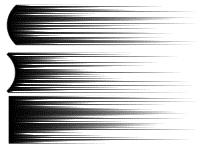
\includegraphics[width=13.9em]{MotionWindInoFunction1LengthWindA}}
\put(142,-171.5){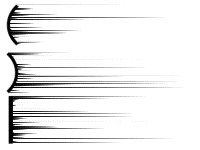
\includegraphics[width=13.9em]{MotionWindInoFunction1LengthWindB}}
\put(284.5,-200){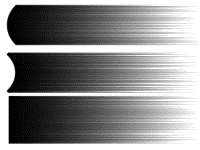
\includegraphics[width=13.9em]{MotionWindInoFunction1LengthWindC}}
\put(209,-16.5){\normalsize{Bias is 0.1}}
\put(351,-45){\normalsize{Bias is 10}}
\end{picture}\\[12.6em]

\normalsize
\noindent Motion Wind 図2 \ \ Force Wind

\large
\noindent \begin{picture}(0,0)
\linethickness{0.01em}
\put(1,-198.5){\line(1,0){198}}
\put(9,-200.5){\line(0,1){62}}
\drawline[0](9,-143)(193,-198.5)
\spline(9,-143)(129,-150)(188,-180)(195,-198.5)
\spline(9,-143)(20,-168.5)(85,-192.5)(193,-198.5)

\put(0.5,-135){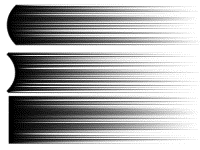
\includegraphics[width=13.9em]{MotionWindInoFunction2MotionWindA}}
\put(142,-171.5){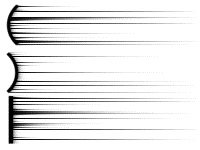
\includegraphics[width=13.9em]{MotionWindInoFunction2MotionWindB}}
\put(284.5,-200){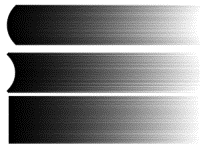
\includegraphics[width=13.9em]{MotionWindInoFunction2MotionWindC}}
\put(209,-16.5){\normalsize{Bias is 0.1}}
\put(351,-45){\normalsize{Bias is 10}}
\end{picture}\\[12.65em]

\normalsize
\noindent Motion Wind 図3 \ \ Density Wind

\large
\noindent \begin{picture}(0,0)
\linethickness{0.01em}
\put(1,-198.5){\line(1,0){198}}
\put(9,-200.5){\line(0,1){62}}
\drawline[0](9,-143)(193,-198.5)
\drawline[0](9,-166.5)(193,-198.5)
\drawline[0](9,-192)(193,-198.5)

\put(0.5,-135){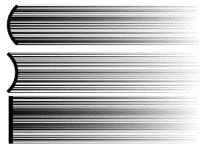
\includegraphics[width=13.9em]{MotionWindInoFunction3DensityWindA}}
\put(142,-171.5){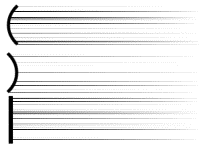
\includegraphics[width=13.9em]{MotionWindInoFunction3DensityWindB}}
\put(284.5,-200){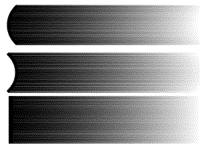
\includegraphics[width=13.9em]{MotionWindInoFunction3DensityWindC}}
\put(209,-16.5){\normalsize{Bias is 0.1}}
\put(351,-45){\normalsize{Bias is 10}}
\end{picture}

\newpage

\thispagestyle{empty}

\ \vspace{-0.1em}
\par
\large
\noindent \hskip 10.5em Length Min equal Max Wind\\[-0.15em]
\normalsize
Motion Wind 図4 \ \ Force is 1 and Density is 1

\large
\noindent \begin{picture}(0,0)
\put(28.5,-132){
\includegraphics[width=13.9em]{MotionWindInoFunction4}}
\end{picture}\\[7.6em]

\large
\noindent \hskip 10.5em Length Min equal Max Wind\\[-0.15em]
\normalsize
Motion Wind 図5 \ \ Force is 0.1

\large
\noindent \begin{picture}(0,0)
\put(28.5,-132){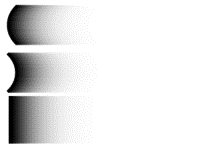
\includegraphics[width=13.9em]{MotionWindInoFunction5}}
\end{picture}\\[7.6em]

\large
\noindent \hskip 10.5em Length Min equal Max Wind\\[-0.15em]
\normalsize
Motion Wind 図6 \ \ Density is 0.2

\large
\noindent \begin{picture}(0,0)
\put(28.5,-132){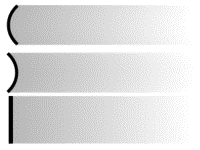
\includegraphics[width=13.9em]{MotionWindInoFunction6}}
\end{picture}\\[7.4em]

\normalsize
\noindent Motion Wind 図7 \ \ Length Wind and Force is 10

\large
\noindent \begin{picture}(0,0)
\put(28.5,-132){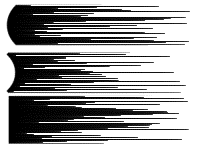
\includegraphics[width=13.9em]{MotionWindInoFunction7}}
\end{picture}

\end{document}